(一)必考题:共 129 分。
\question[6] (6分)某同学用伏安法测量一阻值为几十欧姆的电阻R,所用电压表的内阻为$1kΩ,$电流表内阻为$0.5Ω.$该同学采用两种测量方案,一种是将电压表跨接在图(a)所示电路的$O、P$两点之间,另一种是跨接在$0、Q$两点之间.测量得到如图(b)所示的两条$U-I$图线,其中U与I分别为电压表和电流表的示数.
\begin{center}
    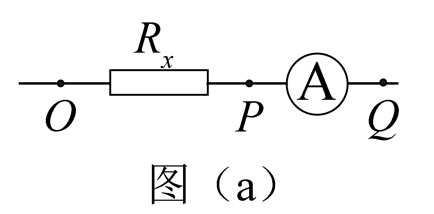
\includegraphics[]{img/image10.png}
\end{center}
回答下列问题:

(1)图(b)中标记为I的图线是采用电压表跨接在\key{O、P}(填$"O$、$P"$或$"O$、$Q")$两点的方案测量得到的.
\begin{center}
    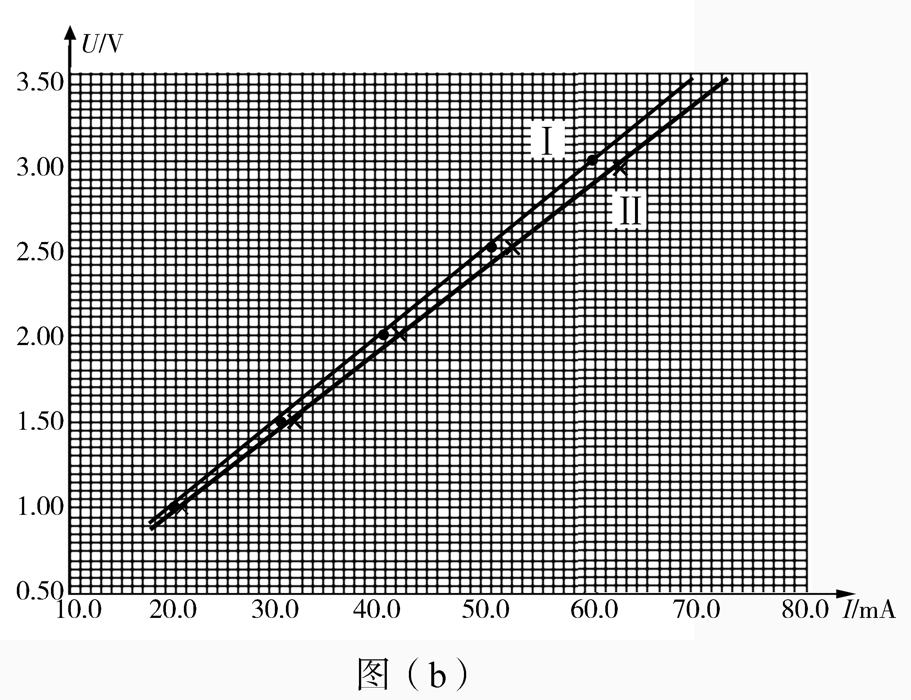
\includegraphics[]{img/image11.png}
\end{center}
(2)根据所用实验器材和图(b)可判断,由图线\key{\uppercase\expandafter{\romannumeral1}}(填$"$\uppercase\expandafter{\romannumeral1}$"$或$"$\uppercase\expandafter{\romannumeral2}$"$)得到的结果更接近待测电阻的真实值,结果为\key{50.5}$Ω$(保留1位小数).

(3)考虑到实验中电表内阻的影响,需对(2)中得到的结果进行修正,修正后待测电阻的阻值为\key{50.0}Ω(保留1位小数).



\newpage
\question[6] (9分)某同学用如图所示的实验装置验证动量定理,所用器材包括:气垫导轨、滑块(上方安装有宽度为d的遮光片)、两个与计算机相连接的光电门、砝码盘和砝码等.

实验步骤如下:
\begin{center}
    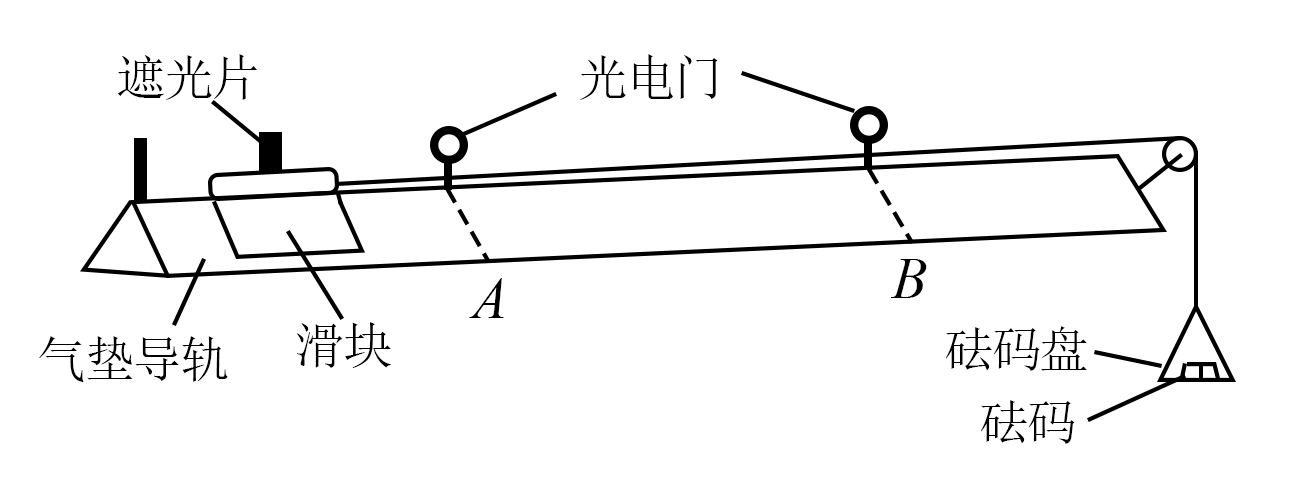
\includegraphics[]{img/image12.png}
\end{center}
(1)开动气泵,调节气垫导轨,轻推滑块,当滑块上的遮光片经过两个光电门的遮光时间\key{大约相等}时,可认为气垫导轨水平;

(2)用天平测砝码与砝码盘的总质量$m_1$、滑块(含遮光片)的质量$m_2$;

(3)用细线跨过轻质定滑轮将滑块与砝码盘连接,并让细线水平拉动滑块;

(4)令滑块在砝码和砝码盘的拉动下从左边开始运动,和计算机连接的光电门能测量出遮光片经过$A$、$B$两处的光电门的遮光时间$Δt_1$、$Δt_2$及遮光片从A运动到B所用的时间$t_{12}$;

(5)在遮光片随滑块从A运动到B的过程中,如果将砝码和砝码盘所受重力视为滑块所受拉力,拉力冲量的大小$I=$\key{$m_1gt_{12}$},滑块动量改变量的大小$Δp=$\key{$m_2(\frac{d}{\Delta t_2}-\frac{d}{\Delta t_1})$};(用题中给出的物理量及重力加速度g表示)

(6)某次测量得到的一组数据为$:d=1.000cm,m_1=1.50×10^{-2}kg,m_2=0.400kg,Δt_1=3.900×10^{-2}s,Δt_2=1.270×10^{-2}s,t_{12}=1.50s,$取$g=9.80m/s^2.$计算可得$I=$\key{0.221}$N·s,Δp=$\key{0.212}$kg∙m·s^{-1};$(结果均保留3位有效数字)

(7)定义$\delta=|\frac{I-\Delta p}{I}|\times 100\%$本次实验$δ=$\key{4}\%(保留1位有效数字).


\question[6] $(12$分)我国自主研制了运$-20$重型运输机.飞机获得的升力大小F可用$F=kv^2$描写,k为系数;ν是飞机在平直跑道上的滑行速度,F与飞机所受重力相等时的v称为飞机的起飞离地速度,已知飞机质量为$1.21×10^5kg$时,起飞离地速度为$66m/s;$装载货物后质量为$1.69×10^5kg﹐$装载货物前后起飞离地时的k值可视为不变.

(1)求飞机装载货物后的起飞离地速度;

(2)若该飞机装载货物后,从静止开始匀加速滑行$1521m$起飞离地,求飞机在滑行过程中加速度的大小和所用的时间.
\begin{solution}{4cm}
(1)$v_2=78m/s$

(2)$a=2.0m/s$\quad $t=39s$
\end{solution}
\newpage
\question[6] $(20$分)在一柱形区域内有匀强电场,柱的横截面积是以O为圆心,半径为R的圆$,AB$为圆的直径,如图所示.质量为m,电荷量为$q(q>0)$的带电粒子在纸面内自A点先后以不同的速度进入电场,速度方向与电场的方向垂直.已知刚进入电场时速度为零的粒子,自圆周上的C点以速率$v_0$穿出电场$,AC$与AB的夹角$θ=60^∘.$运    动中粒子仅受电场力作用.

(1)求电场强度的大小;

(2)为使粒子穿过电场后的动能增量最大,该粒子进入电场时的速度应为多大?

(3)为使粒子穿过电场前后动量变化量的大小为$mv_0,$该粒子进入电场时的速度应为多大?
\begin{center}
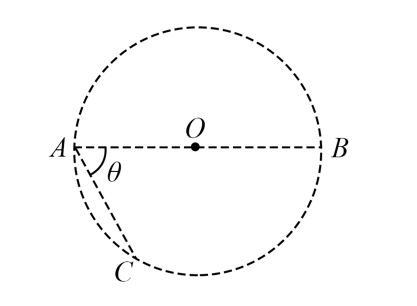
\includegraphics[]{img/image13.png}
\end{center}
\begin{solution}{4cm}
    (1)$E=\frac{mv_0^2}{2qR}$
    
    (2)$v_1=\frac{\sqrt{2}}{4}v_0$

    (3)$v=\frac{\sqrt{3}}{2}v_0$
\end{solution}
\newpage
(二)选考题:共 45 分。请考生从 2 道物理题、2 道化学题、2 道生物题中每科任选一题作答。如果多做, 则每科按所做的第一题计分。
\question[6] [物理——选修$3-3](15$分)

(1)(5分)分子间作用力F与分子间距r的关系如图所示$,r=r_1$时$,F=0.$分子间势能由r决定,规定两分子相距无穷远时分子间的势能为零.若一分子固定于原点O,另一分子从距O点很远处向O点运动,在两分子间距减小到$r_2$的过程中,势能\key{减小}(填"减小"不变"或"增大$");$在间距由$r_2$减小到$r_1$的过程中,势能\key{减小}(填"减小""不变"或"增大$");$在间距等于$r_1$处,势能\key{小于}(填"大于""等于"或"小于")零.
\begin{center}
    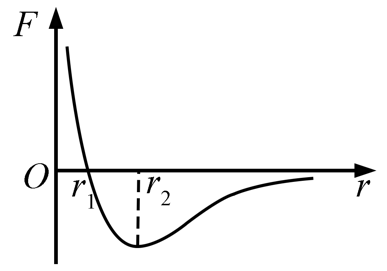
\includegraphics[]{img/image14.png}
\end{center}
(2)(10分)甲、乙两个储气罐储存有同种气体(可视为理想气体).甲罐的容积为V,罐中气体的压强为p;乙罐的容积为$2V,$罐中气体的压强为$\frac{1}{2}p.$现通过连接两罐的细管把甲罐中的部分气体调配到乙罐中去,两罐中气体温度相同且在调配过程中保持不变,调配后两罐中气体的压强相等.求调配后

(i)两罐中气体的压强

(ii)甲罐中气体的质量与甲罐中原有气体的质量之比.
\begin{solution}{4cm}
    (i)$p^\prime=\frac{2}{3}p$

    (ii)$k=\frac{2}{3}$
\end{solution}
\newpage
\question[6] [物理——选修$3-4](15$分)

(1)(5分)在下列现象中,可以用多普勒效应解释的有\key{BCE}。(填正确答案标号.选对1个得2分,选对2个得4分,选对3个得5分;每选错1个扣3分,最低得分为0分)

A.雷雨天看到闪电后,稍过一会儿才能听到雷声

B.超声波被血管中的血流反射后,探测器接收到的超声波频率发生变化

C.观察者听到远去的列车发出的汽笛声,音调会变低

D.同一声源发出的声波,在空气和水中传播的速度不同

E.天文学上观察到双星(相距较近、均绕它们连线上某点做圆周运动的两颗恒星)光谱随时间的周期性变化

(2)(10分)一振动片以频率f做简谐振动时,固定在振动片上的两根细杆同步周期性地触动水面上a、b两点,两波源发出的波在水面上形成稳定的干涉图样.c是水面上的一点,a、b、c间的距离均为l,如图所示.已知除c点外,在ac连线上还有其他振幅极大的点,其中距c最近的点到c的距离为$\frac{3}{8}l.$求:
\begin{center}
    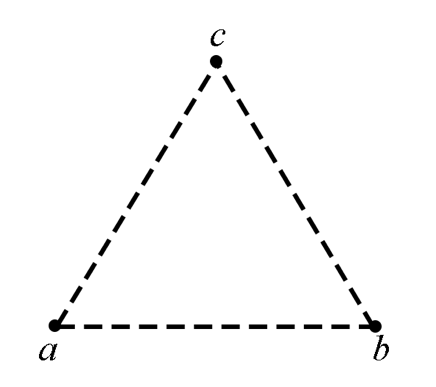
\includegraphics[]{img/image15.png}
\end{center}
(i)波的波长

(ii)波的传播速度。
\begin{solution}{4cm}
    (i)$\lambda=\frac{1}{4}l$

    (ii)$v=\frac{fl}{4}$
\end{solution}

